\documentclass{standalone}

\usepackage{tikz}
\usetikzlibrary{calc}

\begin{document}

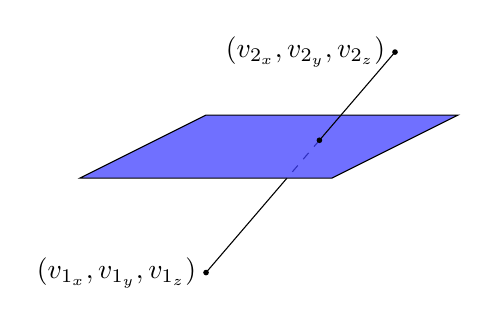
\begin{tikzpicture}[scale=0.8]

\coordinate (O)  at (0,0);
\coordinate (P1) at (-3,-0.5);
\coordinate (P2) at ($(P1)+(2,1)$);
\coordinate (P3) at ($(P2)+(4,0)$);
\coordinate (P4) at ($(P3)+(-2,-1)$);
\coordinate[label=left:{$(v_{1_x},v_{1_y},v_{1_z})$}] (V1) at (-1,-2);
\coordinate[label=left:{$(v_{2_x},v_{2_y},v_{2_z})$}] (V2) at ($(V1)+(3,3.5)$);
\coordinate (I) at ($(V2)!0.4!(V1)$);

\draw[dashed] (I)--($(I)!0.29!(V1)$);
\filldraw[black, fill=blue!75!white, fill opacity=0.75] (P1)--(P2)--(P3)--(P4)--cycle;
\draw (V2)--(I);
\draw ($(I)!0.29!(V1)$)--(V1);

\foreach \pt in {V1,V2,I}{
	\draw[fill=black] (\pt) circle (1pt);
}

\end{tikzpicture}

\end{document}